\documentclass[10pt]{beamer}

\usetheme{metropolis}
\usepackage{appendixnumberbeamer}

\usepackage{booktabs}
\usepackage[scale=2]{ccicons}

\usepackage{pgfplots}
\usepgfplotslibrary{dateplot}

\usepackage{listings}
\lstset{language=R}

\usepackage{color}
\definecolor{mygreen}{rgb}{0,0.6,0}
\definecolor{mygray}{rgb}{0.5,0.5,0.5}
\definecolor{mymauve}{rgb}{0.58,0,0.82}

\lstset{ %
  basicstyle=\footnotesize,        % the size of the fonts that are used for the code
  breakatwhitespace=false,         % sets if automatic breaks should only happen at whitespace
  breaklines=true,                 % sets automatic line breaking
  captionpos=b,                    % sets the caption-position to bottom
  commentstyle=\color{mygreen},    % comment style
  deletekeywords={...},            % if you want to delete keywords from the given language
  escapeinside={\%*}{*)},          % if you want to add LaTeX within your code
  extendedchars=true,              % lets you use non-ASCII characters; for 8-bits encodings only, does not work with UTF-8
  frame=single,	                   % adds a frame around the code
  keepspaces=true,                 % keeps spaces in text, useful for keeping indentation of code (possibly needs columns=flexible)
  keywordstyle=\color{blue},       % keyword style
  language=Octave,                 % the language of the code
  otherkeywords={*,...},           % if you want to add more keywords to the set
  numbers=left,                    % where to put the line-numbers; possible values are (none, left, right)
  numbersep=5pt,                   % how far the line-numbers are from the code
  numberstyle=\tiny\color{mygray}, % the style that is used for the line-numbers
  rulecolor=\color{black},         % if not set, the frame-color may be changed on line-breaks within not-black text (e.g. comments (green here))
  showspaces=false,                % show spaces everywhere adding particular underscores; it overrides 'showstringspaces'
  showstringspaces=false,          % underline spaces within strings only
  showtabs=false,                  % show tabs within strings adding particular underscores
  stepnumber=1,                    % the step between two line-numbers. If it's 1, each line will be numbered
  stringstyle=\color{mymauve},     % string literal style
  tabsize=2,	                   % sets default tabsize to 2 spaces
  title=\lstname                   % show the filename of files included with \lstinputlisting; also try caption instead of title
}

\usepackage{xspace}
\newcommand{\themename}{\textbf{\textsc{metropolis}}\xspace}

\metroset{block=fill}

\title{Reproducible Research}
\subtitle{}
\date{18 March 2016}
\author{
    \href{mailto:christopher.gandrud@city.ac.uk}{Christopher Gandrud}
}
\institute{SG1022, City University London}
% \titlegraphic{\hfill\includegraphics[height=1.5cm]{logo.pdf}}

\begin{document}

\maketitle

\begin{frame}{Table of contents}

    \begin{itemize}
        \item \textbf{What} is research?

        \item \textbf{What} is reproducible research?

        \item \textbf{Why} do we need reproducible research

        \item \textbf{How} to do really reproducible research
    \end{itemize}

\end{frame}

\section{What is reproducible research?}

\begin{frame}{What is research?}

    \begin{center}
        {\large{\emph{Is this research?}}}

        \vspace{0.5cm}

        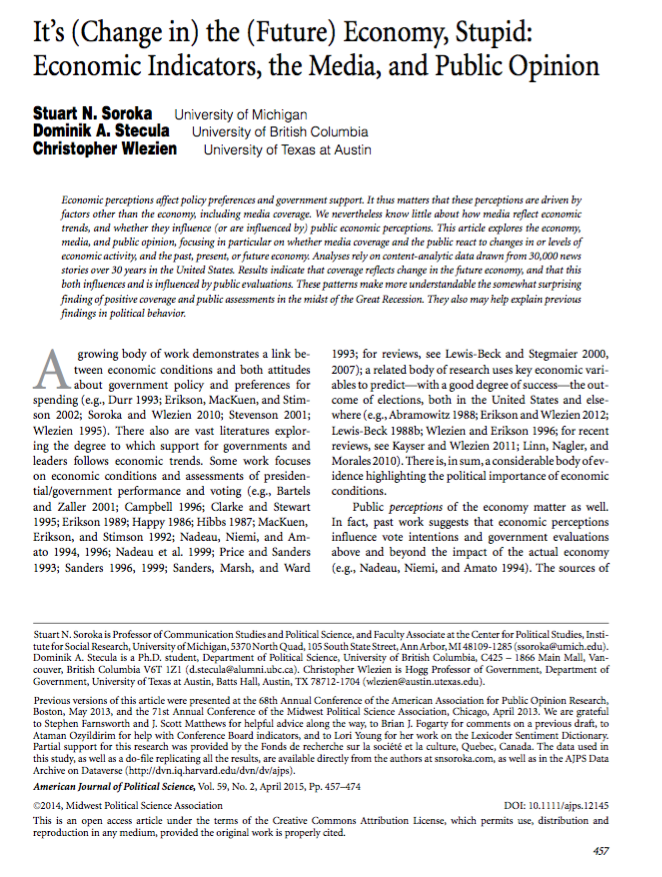
\includegraphics[scale=0.2]{img/journal_ss.png}
    \end{center}
\end{frame}

\begin{frame}{What is research?}

    \begin{center}
        {\large{\emph{Is this research?}}}

        \vspace{0.5cm}

        
\includegraphics[scale=0.2]{img/cox.png}
    \end{center}
\end{frame}

\begin{frame}{Are they research?}

    \begin{alertblock}{No}
        Papers, articles, slideshows, talks, books are the {\large{\textbf{advertising, not the research}}}.
    \end{alertblock}

\end{frame}

\begin{frame}{Are they research?}

    \begin{alertblock}{No}
        Papers, articles, slideshows, talks, books are the {\large{\textbf{advertising, not the research}}}.
    \end{alertblock}

\end{frame}


\begin{frame}{Are they research?}


    Papers, articles, slideshows, talks, books are the {\large{\textbf{advertising, not the research}}}.

    \vspace{1cm}

    \begin{block}{What are they?}
        \textbf{Presentation documents} \emph{announce} select findings and \emph{tries to convince} us that they are correct (Mesirov 2010).
    \end{block}
\end{frame}

\begin{frame}{What is research?}

    Quantitative social science research involves the \textbf{procedures} and \textbf{choices} researchers make to gather data, process it, and analysis it in order to address their research questions.

    \vspace{1cm}

    For {\large{computational research}}, this includes ``the {\large{full software environment, code, and data}} that produced the results'' (Donoho 2010, 3015).

\end{frame}

\begin{frame}
    \begin{center}
        {\large{We need to make available our research, not just the advertising!}}
    \end{center}
\end{frame}


\section{What is reproducible research?}

\begin{frame}{Replicability}

    If we make the research available, not just the advertising, then it will be {\large{more likely}} that other researchers can replicate our work.

    \vspace{1cm}

    \begin{exampleblock}{Replicable Research}
        When there is \emph{sufficient information} available for \emph{independent researchers} to make the \emph{same findings}, using the \emph{same procedures} with \emph{new data}.
    \end{exampleblock}

\end{frame}

\begin{frame}{But\ldots}

    Sometimes full replications \textbf{are not feasible} because:

    \begin{itemize}
        \item \emph{limited resources} for gathering new data (e.g. very expensive to build another Large Hadron Collider),

        \vspace{0.5cm}

        \item the original research already \emph{sampled the universe} of cases.
    \end{itemize}

    \vspace{0.5cm}

    {\large{So\ldots}}

\end{frame}

\begin{frame}{Reproducibility}

    \begin{exampleblock}{Reproducible Research}
        When there is sufficient information available for independent researchers to make the same findings, using the same procedures with the \emph{same data}.
    \end{exampleblock}

\end{frame}

\begin{frame}{Reproducibility}

    \begin{exampleblock}{Really Reproducible Computational Research}
        ``\ldots the \textbf{data and code} used to make a finding are available and they are sufficient for an independent researcher to recreate the finding'' (Peng 2011, 1226)
    \end{exampleblock}

\end{frame}

\begin{frame}{Reproducible and Replicable}

    Reproducible research \textbf{enhances} replicability.

    \begin{itemize}
        \item Reproducible research is a precondition for replicable research.

        \vspace{0.5cm}

        \item Reproducibility is a `second best' if attempting a replication is not possible.

        \vspace{0.5cm}

        \item If it is \textbf{easy} to reproduce your work, more likely that someone else will be able to \textbf{replicate} it.
    \end{itemize}

\end{frame}

\begin{frame}{Reproducible and Replicable}

    \begin{alertblock}{Important!}
        ``\textbf{A study can be reproducible and still be wrong}'' (Peng 2014)

        \vspace{0.5cm}

        E.g. a finding that is statistically significant in one study may remain statistically significant when reproduced using the original data/code, but replication studies are unable to find a similar result.

        \vspace{0.5cm}

        The original finding could just have been \textbf{noise}.
    \end{alertblock}

\end{frame}

\section{Why reproducible research?}

\begin{frame}{For science}

    A \alert{core tenant} of science: Scientific conclusions that are \textbf{not replicable} should be \textbf{abandoned or modified} ``when confronted with more complete or reliable \ldots evidence''

{\tiny{APS \url{http://www.aps.org/policy/statements/99_6.cfm}}}

\end{frame}

\begin{frame}{Examples: World Values Survey}

    \textbf{Background:} the World Values Survey is a large, repeated cross-national survey of political and social values.

    \textbf{Original research finding:}

    \begin{figure}
        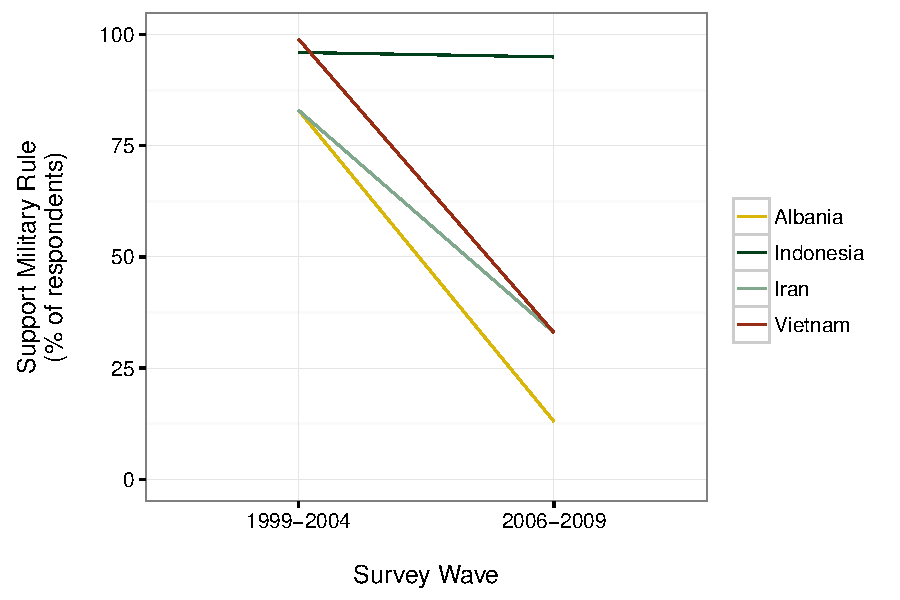
\includegraphics[scale=0.5]{img/wvs_compare.pdf}
    \end{figure}

\end{frame}

\begin{frame}

    \begin{center}
        {\large{Why did support for military rule decline so much in Albania, Iran and Vietnam in only a few years?}}
    \end{center}

\end{frame}




\section{How to do really reproducible research}


\begin{frame}{Linking Presentation to Research}

    To be able to {\large{\textbf{evaluate findings}}} in a presentation document, it needs to be {\large{\textbf{closely linked}}} to the research.

    \vspace{1cm}

    Need to \alert{fully document} the steps we took and the rationale for these steps.

    \begin{itemize}
        \item Documentation \emph{both} in the presentation document (usually discussion of general steps) and ``appendix'' files (e.g. source code, survey questionnaires, raw data).
    \end{itemize}

\end{frame}

\begin{frame}

    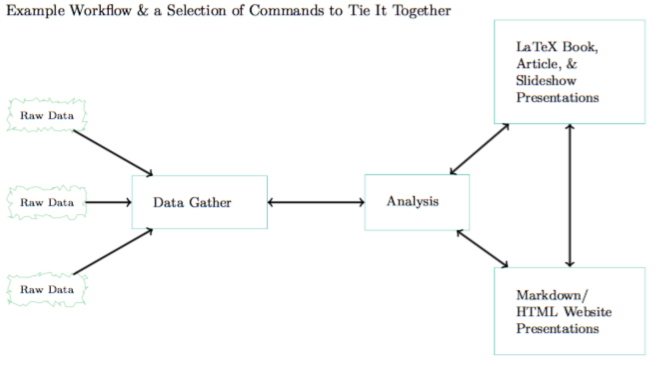
\includegraphics[scale=0.3]{img/workflow.png}

{\tiny{Gandrud (2015, 21)}}
\end{frame}



\begin{frame}[fragile]{Metropolis}


    \begin{lstlisting}
    # A comment
    library(dplyr)
    test <- mean(x, na.rm = T)
    \end{lstlisting}


\end{frame}



\end{document}
